\documentclass[tikz,border=5pt]{standalone}
\usepackage[T1]{fontenc}
\usepackage{lmodern,amsmath,amssymb}
\usetikzlibrary{arrows.meta,calc,positioning,fit,backgrounds,shapes.geometric,matrix,decorations.pathreplacing,patterns}
\definecolor{ink}{gray}{0.08}
\definecolor{wash}{gray}{0.965}
\definecolor{soft}{gray}{0.45}
\tikzset{box/.style={draw=ink,line width=.65pt,fill=white,align=center,inner sep=4pt,outer sep=0pt,font=\small},flow/.style={draw=ink,line width=.65pt,-{Latex[length=1.8mm,width=1.3mm]},rounded corners=2pt},annotation/.style={font=\scriptsize,text=soft,align=center},groupbox/.style={draw=soft,dashed,line width=.45pt,fill=wash}}
\begin{document}
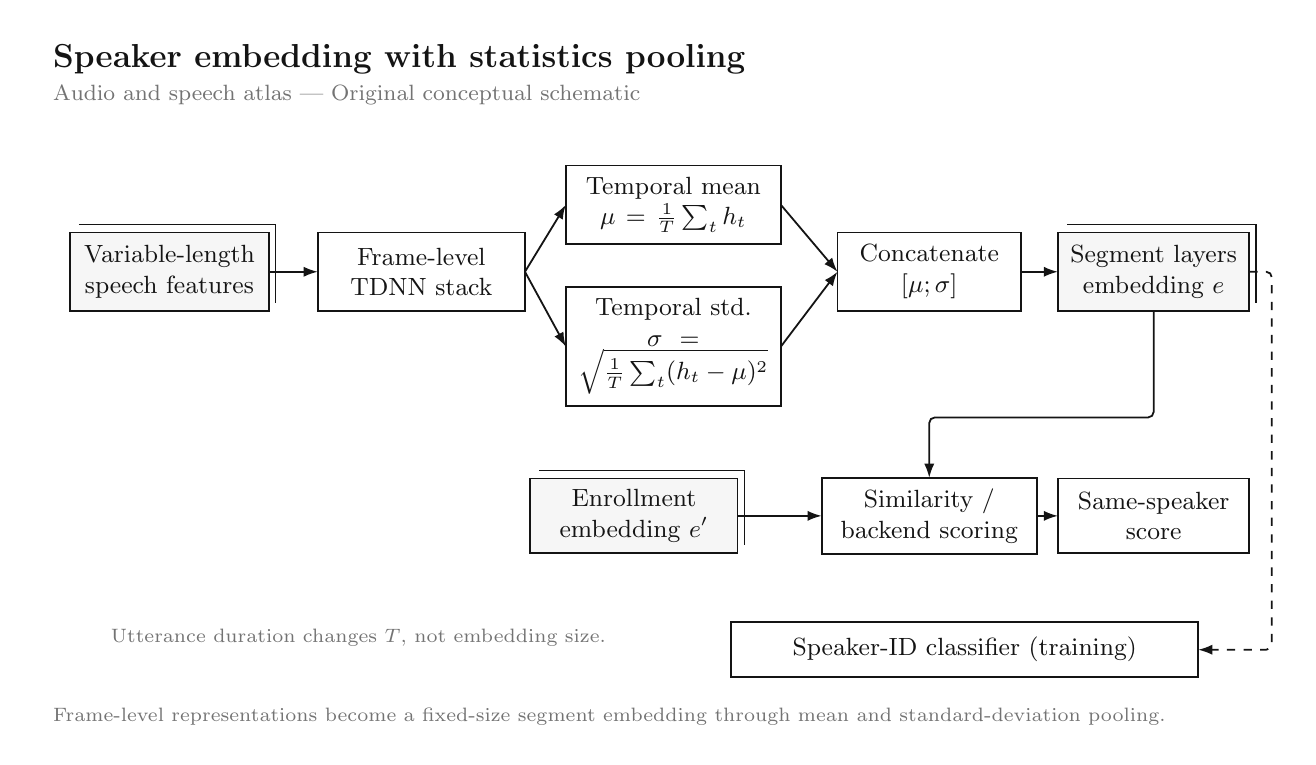
\begin{tikzpicture}[x=1cm,y=-1cm,font=\rmfamily,text=ink]

\path[use as bounding box] (0,0) rectangle (16,9);
\node[anchor=west,font=\large\bfseries] at (.2,.4) {Speaker embedding with statistics pooling};
\node[anchor=west,font=\footnotesize,text=soft] at (.2,.85) {Audio and speech atlas | Original conceptual schematic};
\begin{pgfonlayer}{background}
\end{pgfonlayer}
\node[box,fill=wash,minimum width=2.5cm,minimum height=1.0cm,text width=2.25cm] (features) at (1.8,3.1) {Variable-length\\speech features};
\draw[ink,line width=.4pt] (0.65,2.5) -- (3.15,2.5) -- (3.15,3.5);
\node[box,minimum width=2.6cm,minimum height=1.0cm,text width=2.35cm] (tdnn) at (5.0,3.1) {Frame-level\\TDNN stack};
\node[box,minimum width=2.7cm,minimum height=1.0cm,text width=2.45cm] (mean) at (8.2,2.25) {Temporal mean\\$\mu=\frac1T\sum_t h_t$};
\node[box,minimum width=2.7cm,minimum height=1.0cm,text width=2.45cm] (std) at (8.2,4.05) {Temporal std.\\$\sigma=\sqrt{\frac1T\sum_t(h_t-\mu)^2}$};
\node[box,minimum width=2.3cm,minimum height=1.0cm,text width=2.05cm] (concat) at (11.45,3.1) {Concatenate\\$[\mu;\sigma]$};
\node[box,fill=wash,minimum width=2.4cm,minimum height=1.0cm,text width=2.15cm] (embed) at (14.3,3.1) {Segment layers\\embedding $e$};
\draw[ink,line width=.4pt] (13.200000000000001,2.5) -- (15.6,2.5) -- (15.6,3.5);
\node[box,fill=wash,minimum width=2.6cm,minimum height=0.95cm,text width=2.35cm] (enroll) at (7.7,6.2) {Enrollment\\embedding $e'$};
\draw[ink,line width=.4pt] (6.5,5.625000000000001) -- (9.1,5.625000000000001) -- (9.1,6.575);
\node[box,minimum width=2.7cm,minimum height=0.95cm,text width=2.45cm] (score) at (11.45,6.2) {Similarity /\\backend scoring};
\node[box,minimum width=2.4cm,minimum height=0.95cm,text width=2.15cm] (decision) at (14.3,6.2) {Same-speaker\\score};
\node[box,minimum width=5.9cm,minimum height=0.7cm,text width=5.65cm] (train) at (11.9,7.9) {Speaker-ID classifier (training)};
\begin{pgfonlayer}{background}
\draw[flow] (features.east) -- (tdnn.west);
\draw[flow] (tdnn.east) -- (mean.west);
\draw[flow] (tdnn.east) -- (std.west);
\draw[flow] (mean.east) -- (concat.west);
\draw[flow] (std.east) -- (concat.west);
\draw[flow] (concat.east) -- (embed.west);
\draw[flow] (enroll.east) -- (score.west);
\draw[flow] (embed.south) -- (14.3,4.95) -- (11.45,4.95) -- (score.north);
\draw[flow] (score.east) -- (decision.west);
\draw[flow,dashed] (embed.east) -- (15.8,3.1) -- (15.8,7.9) -- (train.east);
\end{pgfonlayer}
\node[align=center,anchor=center,font=\scriptsize,text=soft,text width=7cm] at (4.2,7.75) {Utterance duration changes \mbox{$T$}, not embedding size.};
\node[anchor=west,align=left,font=\scriptsize,text=soft,text width=15.6cm] at (.2,8.75) {Frame-level representations become a fixed-size segment embedding through mean and standard-deviation pooling.};
\end{tikzpicture}
\end{document}
